\documentclass{beamer}
\usetheme[compress]{Singapore}
%\useoutertheme{miniframes}

% \documentclass{beamer}
%\usetheme{Warsaw}

% Pour les documents en francais...
	\usepackage[latin1]{inputenc}
	\usepackage[french]{babel}
	\usepackage[french]{varioref}
%\usepackage[T1]{fontenc} 

% Math?matiques
	\usepackage{amsmath}

% Caracteres speciaux suppl?mentaires
	\usepackage{latexsym,amsfonts}

% A documenter
	\usepackage{moreverb}

% Macros pour les paquets
	\usepackage{array}  			% N?cessaires pour les tableaux de la macro Excel.

% Outil suppl?mentaire pour les tableaux
	\usepackage{multirow}
	\usepackage{booktabs}
	\usepackage{xcolor} % alternating row colors in table, incompatible avec certains modules
	\usepackage{longtable}
	\usepackage{colortbl}

% Pour ins?rer des graphiques
	\usepackage{graphicx} 			% Graphique simples
	\usepackage{subfigure}			% Graphiques multiples

% Pour ins?rer des couleurs
	\usepackage{color}

% Rotation des objets et des pages
%	\usepackage{rotating}
%	\usepackage{lscape}

% Pour insrer du code source, LaTeX ou SAS par exemple.
	\usepackage{verbatim}
         \usepackage{moreverb}
	\usepackage{listings}
	\lstset{basicstyle=\ttfamily,
  		showstringspaces=false,
  		commentstyle=\color{red},
  		keywordstyle=\color{blue}
	}
	\usepackage{fancyvrb}

%	\lstset{language=SAS,numbers=left}		% Par dfaut le listing est en SAS

% Pour ins?rer des hyperliens
  \usepackage{hyperref}

% American Psychological Association (for bibliographic references).
	\usepackage{apacite}

% Pour l'utilisation des macros
	\usepackage{xspace}

% Pour l'utilisation de notes en fin de document.
%	\usepackage{endnotes}

% Array
%	\usepackage{multirow}
%	\usepackage{booktabs}

% Rotation
%	\usepackage{rotating}

% En t?tes et pieds de pages
%	\usepackage{fancyhdr}
%	\usepackage{lastpage}


% Page layout

% By LaTeX commands
%\setlength{\oddsidemargin}{0cm}
%\setlength{\textwidth}{16cm}
%\setlength{\textheight}{24cm}
%\setlength{\topmargin}{-1cm}
%\setlength{\marginparsep}{0.2cm}

% fancyheader parameters
%\pagestyle{fancy}

%\fancyfoot[L]{{\small Formation \LaTeX, DEPP}}
%\fancyfoot[c]{}
%\fancyfoot[R]{{\small \thepage/\pageref{LastPage}}}

%\fancyhead[L]{}
%\fancyhead[c]{}
%\fancyhead[R]{}

% Pour ins?rer des dessins de Linux
\newcommand{\LinuxA}{\includegraphics[height=0.5cm]{Graphiques/linux.png}}
\newcommand{\LinuxB}{\includegraphics[height=0.5cm]{Graphiques/linux.png}\xspace}

% Macro pour les petits dessins pour les diff?rents OS.
\newcommand{\Windows}{\emph{Windows}\xspace}
\newcommand{\Mac}{\emph{Mac OS X}\xspace}

\newcommand{\Linux}{\emph{Linux}\xspace}
\newcommand{\linux}{\emph{Linux}\xspace}

\newcommand{\GNULinux}{\emph{GNU/Linux}\xspace}
\newcommand{\gnulinux}{\emph{GNU/Linux}\xspace}

\newcommand{\Fedora}{\emph{Feodra}\xspace}
\newcommand{\Ubuntu}{\emph{Ubuntu}\xspace}


\newcommand{\MikTeX}{MiK\tex\xspace}
\newcommand{\latex}{\LaTeX\xspace}


\newcommand{\df}{\emph{data.frame}\xspace}
\newcommand{\liste}{\emph{list}\xspace}
\newcommand{\cad}{c'est-�-dire\xspace}

% Titre
\title{Introduction � GNU/Linux}
\author{Pascal Bessonneau}
\institute{Starinux}
\date{11/2017}

\subtitle{Utilisateurs}


\newcommand{\hreff}[2]{\underline{\href{#1}{#2}\xspace}}

\begin{document}

\begin{frame}
	\maketitle
\end{frame}

\begin{frame}
	\tableofcontents
\end{frame}

% Begin document %%%%%%%%%%%%%%%%%%%%%%%%%%%%%%%%%%%%%%%%%%%%%%%%%%%%%%%%%%%%%%%%%%%%%%%%%%%%%%%%%%

\section{Introduction}

\begin{frame}[containsverbatim]
  \frametitle{Qu'est ce qu'un utilisateur ?}
	
	C'est un compte permettant g�n�ralement une connexion (graphique ou console).
	
	Il est associ� sous UNIX � un num�ro qui est utilis� pour identifier les fichier et les r�pertoires
	
	Il est g�n�ralement associ� � la pr�sence d'un r�pertoire utilisateur qui lui appartient.

\end{frame}

\begin{frame}[containsverbatim]
  \frametitle{Qu'est ce qu'un utilisateur ?}

	Il existe des utilisateurs sp�ciaux qui n'ont pas de r�pertoire et/ou la connexion n'est pas possible.
	
	C'est le cas pour de nombreux serveurs qui fonctionnent ainsi pour des raisons de s�curit�.
	
\end{frame}

\section{Gestion des utilisateurs}

\begin{frame}[containsverbatim]
  \frametitle{Cr�er/supprimer un utilisateur}

	Pour cr�er un utilisateur, il suffit d'utiliser la commande \emph{adduser <utilisateur>} pr�c�d� de \emph{sudo}.
	
	Et apr�s il faut r�pondre aux questions, relativement simple.
	
	En effet la gestion des utilisateurs est r�serv� au super utilisateur.

	Pour supprimer un utilisateur, il faut utiliser \emph{deluser <utilisateur>} et de r�pondre aux questions.
		
\end{frame}

\begin{frame}[containsverbatim]
  \frametitle{Les fichiers de r�f�rence}
	
	Le fichier des utilisateurs est le fichier /etc/passwd.
	
	Le fichier des groupes est le fichier /etc/group.
	
	Le fichier des groupes est plus int�ressant car il permet de voir quels groupes contiennent quels utilisateurs.
	C'est utile par exemple pour copier les droits de l'utilisateur cr�� par d�faut par votre distribution.

	\textcolor{red}{Mais il faut �viter de manipuler directement ces fichiers car s'ils sont corrompus le syst�me d'authentification peut planter}
\end{frame}

\begin{frame}[containsverbatim]
  \frametitle{Gestion des groupes}
	
	Pour ajouter un groupe � un utilisateur, il faut utiliser la commande~:
	\emph{usermod -a -G <groupe> <utilisateur>}.
	
	Pour ajouter un groupe � un utilisateur, il faut utiliser la commande~:
	\emph{gpasswd -d <utilisateur> <group>}.
		
\end{frame}

\begin{frame}[containsverbatim]
  \frametitle{Nota bene}
	
	Les droits sont des num�ros.
	
	Si l'utilisateur pascal est 1001 sur un ordinateur et 1002 sur un autre ordinateur, alors
	si vous �changez les disques les fichiers ne seront pas reconnus comme pascal sur l'un
	ou l'autre des ordinateurs.
		
\end{frame}

\begin{frame}[containsverbatim]
  \frametitle{En mode graphique}
	
	Sous KDE, l'utilitaire KUser permet de le faire graphiquement comme system-config-users sous GNOME.
		
\end{frame}

\begin{frame}[containsverbatim]
  \frametitle{Sous GNOME 3}

\begin{center}
\begin{figure}
 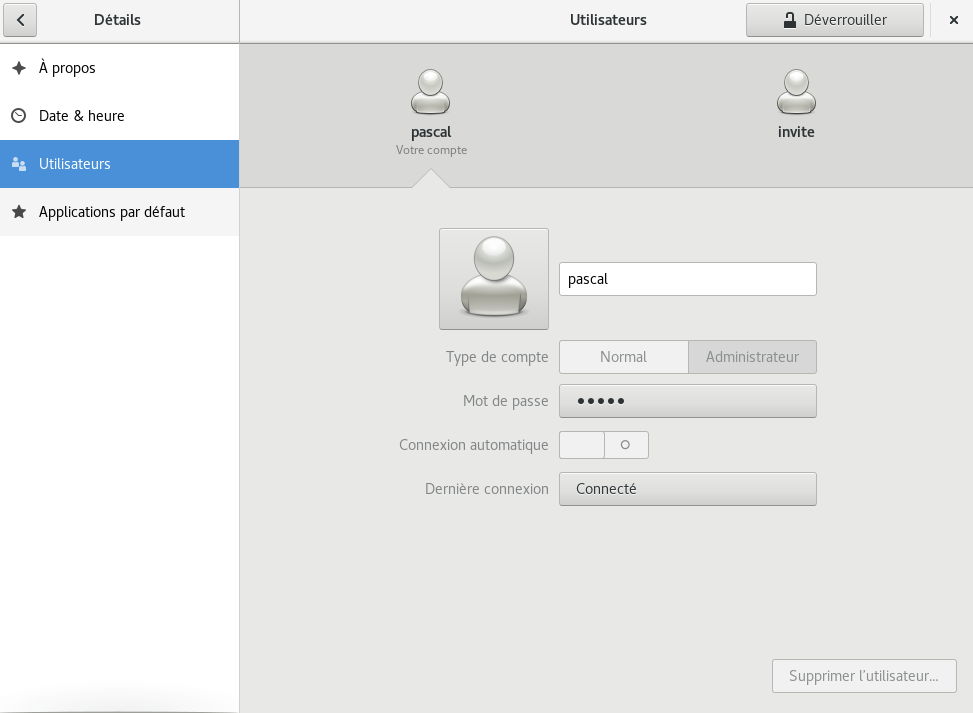
\includegraphics[scale=0.2]{Figures/Selection005}
	\caption{Utilisateurs dans le menu D�tails de l'application Param�tres}
\end{figure}
\end{center}
  
  \end{frame}

\begin{frame}[containsverbatim]
  \frametitle{Sous GNOME 3}

\begin{center}
\begin{figure}
 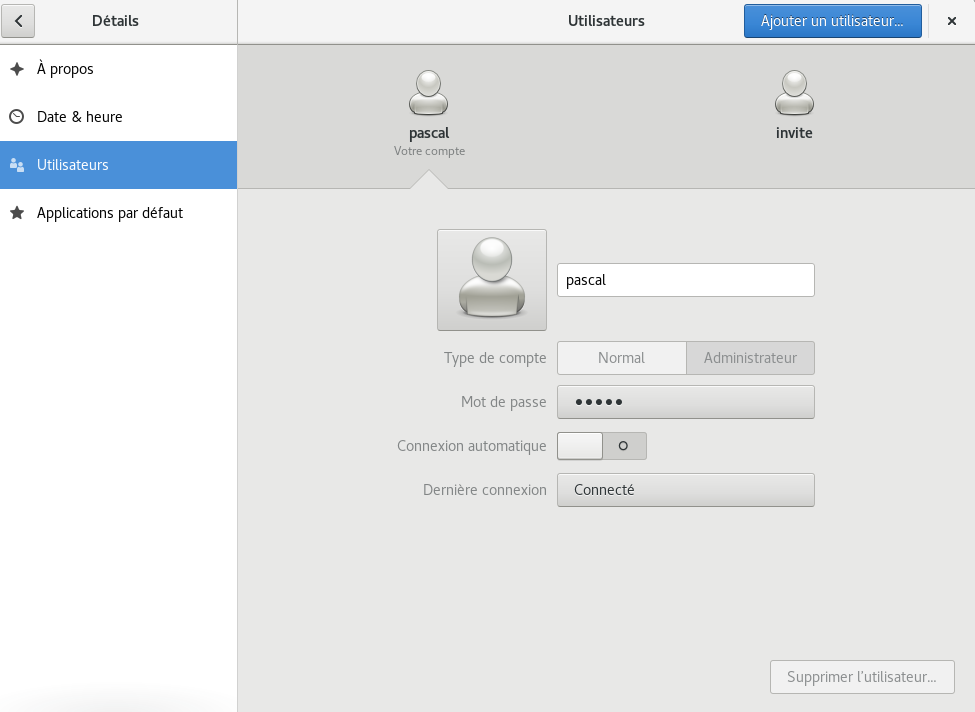
\includegraphics[scale=0.2]{Figures/Selection006}
	\caption{Utilisateurs, d�blocage avec le mot de passe}
\end{figure}
\end{center}
  
  \end{frame}


\begin{frame}[containsverbatim]
  \frametitle{Sous GNOME 3}

\begin{center}
\begin{figure}
 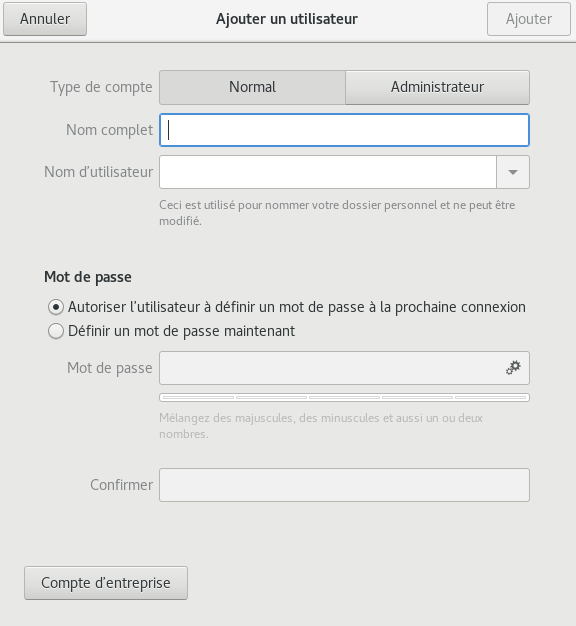
\includegraphics[scale=0.2]{Figures/Selection007}
	\caption{Utilisateurs, nouvel utilisateur}
\end{figure}
\end{center}
  
  \end{frame}

	
\end{document}